\section{Results and Discussion}
System-level simulation was performed with representative AI inference workloads.

\begin{itemize}
  \item \textbf{Standby Power}: $>$30\% reduction by migrating cold data to FeRAM-backed tier.
  \item \textbf{Resume Latency}: reduced to $\mu$s–ms range, enabling instant resume across power cycles.
  \item \textbf{Endurance}: $10^{12}$ writes/year fits within FeRAM capability for checkpoint traffic.
\end{itemize}

\begin{figure}[!t]
\centering
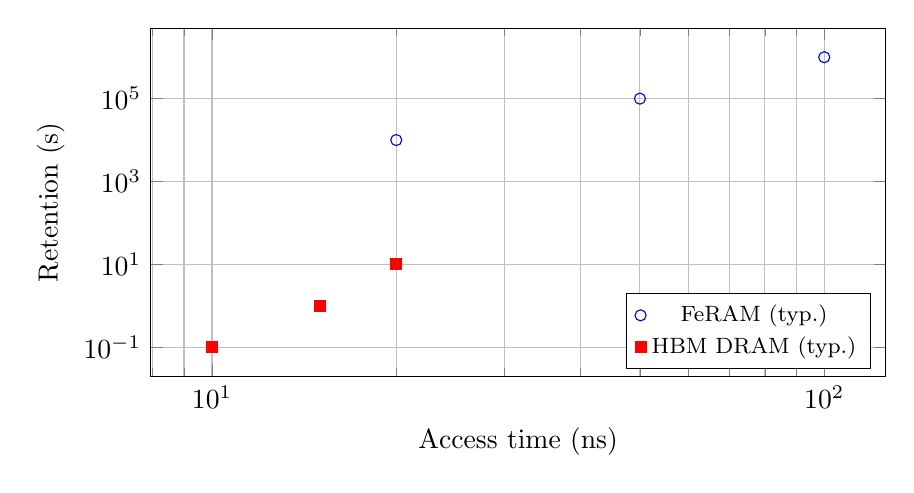
\begin{tikzpicture}
  \begin{loglogaxis}[
    width=0.9\linewidth, height=6cm,
    xlabel={Access time (ns)},
    ylabel={Retention (s)},
    grid=both,
    legend style={at={(0.98,0.02)},anchor=south east,font=\footnotesize}
  ]
    % FeRAM points (blue circles)
    \addplot[only marks, mark=o, blue] coordinates {
      (20,1e4) (50,1e5) (100,1e6)
    };
    \addlegendentry{FeRAM (typ.)}

    % HBM DRAM points (red squares)
    \addplot[only marks, mark=square*, red] coordinates {
      (10,1e-1) (15,1e0) (20,1e1)
    };
    \addlegendentry{HBM DRAM (typ.)}
  \end{loglogaxis}
\end{tikzpicture}
\caption{Access time vs. retention. Red squares: HBM; blue circles: FeRAM.}
\label{fig:retention}
\end{figure}
